%Preambolo
\documentclass[a4paper, 12pt]{article}
\usepackage[T1]{fontenc}
\usepackage[utf8]{inputenc}
\usepackage[italian]{babel}
\usepackage{graphicx}
\usepackage{subcaption}
\usepackage{amsmath}
\usepackage{hyperref} %per i riferimenti
\usepackage{enumitem} %per modificare gli elenchi puntati e le enumerazioni
\usepackage{array}
\usepackage{longtable} %per creare tabelle multipagina
\usepackage{verbatim} %per i commenti multiriga
\usepackage{tabularx}
    %\newcolumntype{L}{>{\raggedright\arraybackslash}X}
    \newcolumntype{b}{>{\hsize=0.76\hsize}X}
    \newcolumntype{s}{>{\hsize=0.22\hsize}X}

%preambolo per inserire codice sql
\usepackage{listings}
\usepackage{color}

%definizione dei colori
\definecolor{codegreen}{rgb}{0,0.6,0}
\definecolor{codegray}{rgb}{0.5,0.5,0.5}
\definecolor{codepurple}{rgb}{0.58,0,0.82}
\definecolor{backcolour}{rgb}{0.95,0.95,0.92}

%definizione dello stile per il linguaggio sql
\lstdefinestyle{sqlstyle}{
    language=sql,
    backgroundcolor=\color{backcolour},   
    commentstyle=\color{codegreen},
    keywordstyle=\color{blue},
    numberstyle=\tiny\color{codegray},
    stringstyle=\color{codepurple},
    basicstyle=\footnotesize\ttfamily,
    breakatwhitespace=true,
    breaklines=true,
    postbreak=\mbox{\space\space\space\space\space\textcolor{red}{$\hookrightarrow$}\space},
    captionpos=b,
    keepspaces=true,
    numbers=left,
    numbersep=5pt,
    showspaces=false,
    showstringspaces=false,
    showtabs=false,
    tabsize=2
}

\begin{document}

%Frontespizio
\begin{titlepage}
\begin{figure}[!htb]
    \centering
    
\includegraphics[keepaspectratio=true, width=0.5\linewidth]{immagini/Federico_II.jpg}
\end{figure}

\begin{center}
    \vspace{10mm}
    \LARGE{Corso di Laurea Triennale in Informatica}
\end{center}

\vspace{10mm}
\begin{center}
    \LARGE{\bf{Documentazione del DataBase per Compagnia di Navigazione\\}}
    \vspace{20mm}
    \Large{Raucci Giovanni N86004635\\}
    \Large{Regina Riccardo N86004614\\}
    \Large{Rossetti Francesco N86004505\\}
\end{center}


\vspace{30mm}


\hrulefill
\\\centering{\large{DICEMBRE 2023}}

\end{titlepage}

\tableofcontents
\newpage

\section{Progettazione Concettuale}
\subsection{Analisi dei Requisiti}
Durante la fase di analisi dei requisiti, l'obiettivo principale è identificare le informazioni chiave necessarie per la realizzazione della struttura del database della compagnia di navigazione. In particolare, si concentrerà sull'individuazione delle entità, delle associazioni tra di esse, e sui vincoli e comportamenti del database.

\begin{quote}
    \textit{"Il sistema si basa sulla conoscenza delle corse offerte dalle compagnie di navigazione. Ogni corsa è offerta da una specifica compagnia di navigazione, che indica il tipo di natante utilizzato. Tra i tipi di natante si distinguono i traghetti (che trasportano persone e automezzi), gli aliscafi e le motonavi (che trasportano entrambe solo passeggeri). Ogni corsa ha cadenza giornaliera, un orario di partenza e un orario di arrivo ma può essere operata solo in alcuni giorni della settimana e solo in alcuni specifici periodi dell’anno. Ad esempio, una compagnia potrebbe operare una corsa di motonave da Mu ad Atlantide soltanto il martedì e il giovedì e nel periodo tra il 15 giugno e il 15 settembre."}
\end{quote}

In base alle specifiche fornite, è possibile identificare diverse entità fondamentali per la struttura del database. Inizialmente, l'entità \textit{CORSAREGOLARE} conterrà le informazioni fondamentali relative alle corse ricorrenti in determinati periodi dell'anno, compresi gli orari di partenza e di arrivo. Inoltre, \textit{CORSASPECIFICA} rappresenterà un'istanza specifica di una corsa regolare e includerà quindi come attributo la data in cui si svolgerà la corsa.

Un'altra entità individuata è il \textit{NATANTE} dotato di nome e suddiviso in tre tipi distinti: \textit{TRAGHETTO}, con posti dedicati sia a passeggeri che a veicoli; \textit{ALISCAFO} e \textit{MOTONAVE}, entrambi progettati solo per passeggeri. Poiché le richieste specificano il vincolo di effettuare ogni corsa solo in determinati periodi dell'anno, l'entità \textit{CORSAREGOLARE} sarà associata ad un'entità \textit{PERIODO} che conterrà una data di inizio e una data di fine periodo in cui la corsa può essere effettuata, inoltre avrà anche un attributo multivalore per indicare i giorni della settimana in cui la corsa è disponibile. Questa scelta di implementazione è motivata dal fatto che ogni corsa può coprire un numero non precisato di periodi.

\begin{quote}
    \textit{"Ogni corsa ha diversi prezzi: un prezzo per il biglietto intero, uno per il biglietto ridotto. Inoltre può esserci un sovrapprezzo per la prenotazione e uno per i bagagli. Ogni corsa è caratterizzata da un porto di arrivo e da uno di partenza: nel caso di corse che abbiano uno scalo intermedio il sistema espone tra le sue corse tutte le singole tratte. Ad esempio, se esiste una corsa tra Mu e Atlantide con scalo a Tortuga, il sistema manterrà tutte e tre le corse da Mu a Tortuga, da Tortuga ad Atlantide e da Mu ad Atlantide. Ogni compagnia di navigazione ha un nome e una serie di contatti (telefono, mail, sito web indirizzi su diversi social)."}
\end{quote}

Per quanto riguarda la gestione dei prezzi, l'entità \textit{CORSAREGOLARE} comprende gli attributi relativi al costo del biglietto intero, eventuali sconti per prezzi ridotti e i sovrapprezzi legati alla prenotazione, ai bagagli o al veicolo che il \textit{CLIENTE} desidera imbarcare.

Dall'altra parte, nell'entità \textit{BIGLIETTO} sono inclusi gli attributi associati alle scelte effettuate dal cliente durante l'acquisto del biglietto, come l'età del passeggero, la prenotazione e l'imbarco di bagagli o veicoli.

L'entità \textit{PORTO} è caratterizzata da attributi come il comune, l'indirizzo e il numero di telefono del porto. Tra l'entità \textit{PORTO} e \textit{CORSAREGOLARE}, esistono diverse relazioni che andranno a mappare per ogni corsa il porto di partenza, di arrivo e quello di un possibile scalo intermedio.

Per quanto riguarda l'entità \textit{COMPAGNIA}, gli attributi comprendono il nome e vari contatti come numeri telefonici, indirizzi email e sito web. Inoltre, considerando la diversità dei social media, i quali potrebbero avere tag distinti, verranno strutturati come un'entità separata \textit{SOCIAL}.

\begin{quote}
    \textit{"Il sistema può essere utilizzato dalle compagnie e dai passeggeri. Le compagnie possono aggiornare le proprie corse oppure segnalare l’annullamento o il ritardo di una singola corsa. Il passeggero può consultare il tabellone delle corse, che contiene tutte le corse da un determinato porto di partenza verso un determinato porto di destinazione, da un giorno e orario di partenza indicato e per le successive 24 ore, eventualmente filtrate in base al tipo di natante scelto o in base al prezzo. Nel tabellone le corse in ritardo o cancellate dovranno comunque essere mostrato con una annotazione che riporti questo evento."}
\end{quote} 

Poiché il sistema prevede l'utilizzo da parte di due categorie distinte di utenti, verrà introdotta una generalizzazione delle classi \textit{COMPAGNIA} e \textit{CLIENTE} nella classe \textit{UTENTE}. Quest'ultima sarà dotata di attributi di login e password per consentire l'autenticazione.

Dal momento che le compagnie hanno la facoltà di aggiornare, cancellare o segnalare ritardi per singole corse, saranno aggiunti due attributi all'entità \textit{CORSASPECIFICA}: uno per i minuti di ritardo e l'altro per indicare se la corsa è stata cancellata o meno.

\begin{quote}
    \textit{"Le compagnie indicano anche la capienza dei natanti utilizzati per quella corsa, in termini di numero di posti per i passeggeri e numero di posti per autoveicoli. I passeggeri possono prenotare una singola corsa solo se il sistema verificherà la presenza di un posto utile. All’atto della prenotazione il sistema dovrà aggiornare il numero dei posti utili in tutte le tratte interessate. Ad esempio, all’atto della prenotazione di due biglietti passeggero e un autoveicolo da Atlantide a Tortuga dovranno essere diminuite le disponibilità di biglietti passeggero ed autoveicolo anche nella tratta da Atlantide a Mu (ma non in quella da Tortuga a Mu)."}
\end{quote}

Siccome è richiesto identificare quanti posti disponibili ci sono, saranno inseriti come attributi nell'entità \textit{CORSASPECIFICA}.
\newpage

\subsection{Schema Concettuale UML}
\begin{figure}[h!]
    \centering
    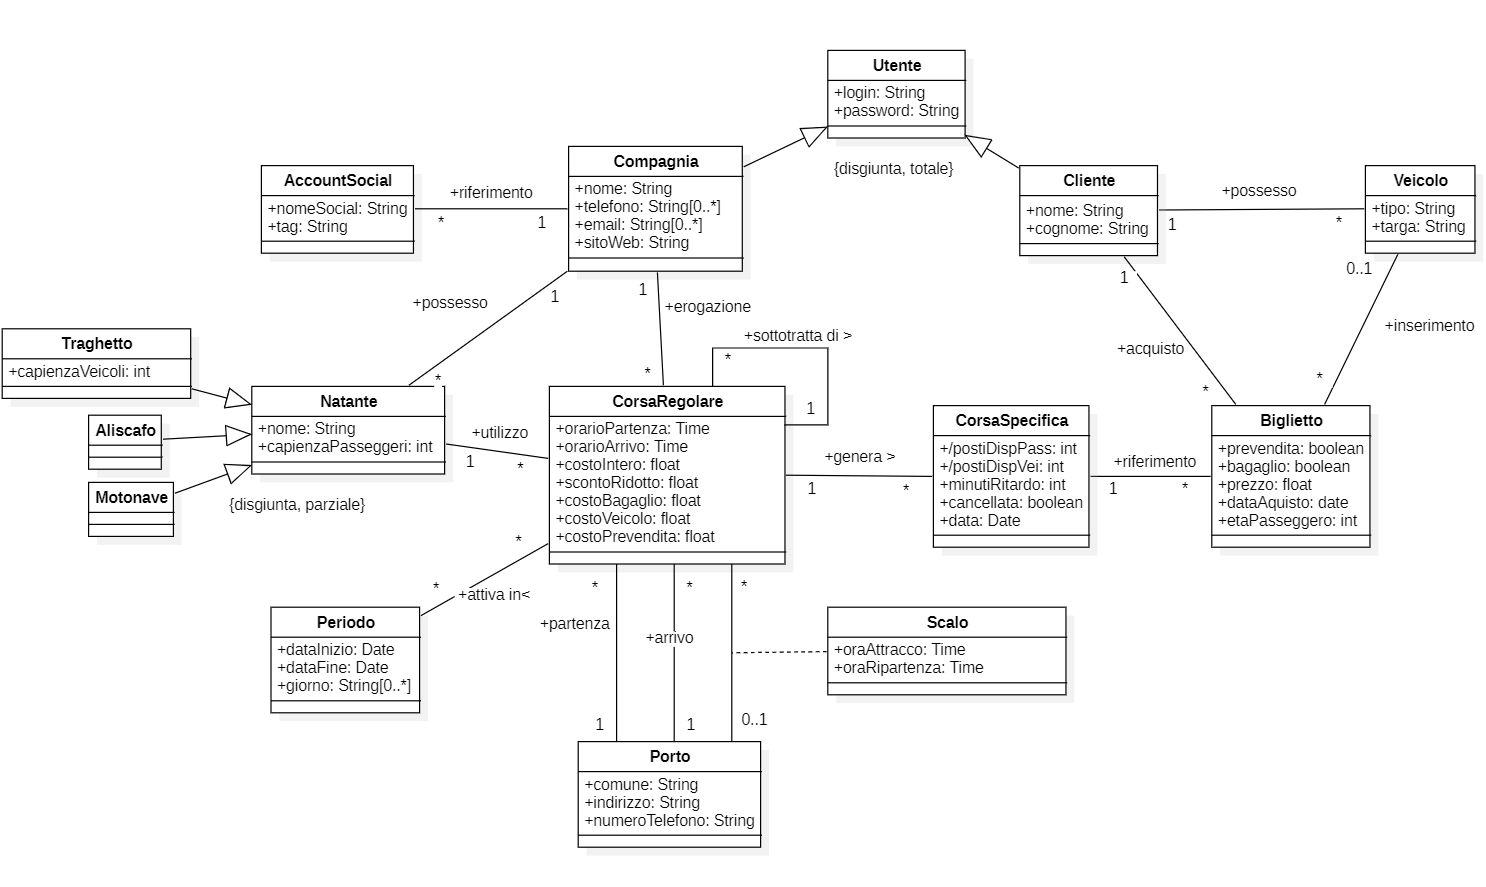
\includegraphics[width = 0.9\textwidth]{immagini/UMLdiagramNonRistrutturato.png}
    \label{UMLNonRistrutturato}
\end{figure}

\subsection{Dizionario delle Classi}

\vspace{4mm}

\begin{longtable}{|| m{0.2\textwidth} | m{0.35\textwidth} | m{0.45\textwidth} ||}
    \hline\hline
     \textbf{Classe} & \textbf{Descrizione} & \textbf{Attributi} \\
     \hline\hline
     \endfirsthead

     \hline
     \textbf{Classe} & \textbf{Descrizione} & \textbf{Attributi} \\
     \hline
     \endhead

     %Utente
     Utente & L'utente fa l'accesso al sistema o come Compagnia per aggiungere o aggiornare le corsa, o come Cliente per consultare le corse disponibili &
     \textbf{login}(String): login identificativo per accedere all'area riservata della compagnia o del cliente
     
     \textbf{password}(String): password per accedere all'area riservata della compagnia o del cliente\\
     \hline

     %Compagnia
     Compagnia & La compagnia di navigazione offre delle corse in traghetto, aliscafo, motonave o altro tra le varie isole  & 
     \textbf{nome}(String): nome della compagnia

     \textbf{numero}(String): numero di telefono della compagnia

     \textbf{indirizzo}(String): indirizzo di posta elettronica della compagnia
     
     \textbf{sitoWeb}(String): link URL al sito web della compagnia\\
     \hline

     %Porto
     Porto & Luogo in cui le imbarcazioni salpano e attraccano &
     \textbf{comune}(String): nome del comune di appartenenza del porto
     
     \textbf{indirizzo}(String): indirizzo presso il quale è situato il porto
     
     \textbf{numeroTelefono}(String): numero telefonico del servizio informazioni\\
     \hline

     %Scalo
     Scalo & Atrracco al porto di un isola intermedia per consentire ad altri passeggeri di arrivare a destinazione & 
     \textbf{OraAttracco}(Timestamp): ora in cui il natante arriva al porto
     
     \textbf{OraRipartenza}(Timestamp): ora in cui il natante riparte
     
     \textbf{costoPrimaTratta}(float): costo della tratta intermedia che va dal porto di partenza al porto di scalo

     \textbf{costoSecondaTratta}(float): costo della tratta intermedia che va dal porto di scalo al porto di arrivo\\
     \hline

     %CorsaRegolare
     CorsaRegolare & Tratta marittima messa a disposizione da una compagnia che collega due isole (o tre se c'è uno scalo) che si ripeterà per determinati periodi e determinati giorni &   
     \textbf{OrarioPartenza}(Time): ora in cui il natante salpa dal porto di partenza e ha inizio la corsa
     
     \textbf{OrarioArrivo}(Time): ora in cui il natante attracca al porto di arrivo e la corsa ha termine
     
     \textbf{costoIntero}(float): costo base della corsa per un adulto senza bagaglio o veicolo
     
     \textbf{scontoRidotto}(float): percentuale di sconto per un biglietto ridotto

     \textbf{costoBagaglio}(float): sovrapprezzo per i clienti che portano un bagaglio

     \textbf{costoVeicolo}(float): sovrapprezzo per i clienti che imbarcano un veicolo

     \textbf{costoPrevendita}(float): sovrapprezzo per i clienti che acquistano il biglietto in prevendita\\
     \hline

     %CorsaSpecifica
     CorsaSpecifica & Istanza specifica di una corsa regolare &
     \textbf{data}(Date): giorno in cui viene effettuata la corsa
     
     \textbf{postiDispPass}(int): numero di posti passeggeri ancora disponibili
     
     \textbf{postiDispVei}(int): numero di posti veicoli ancora disponibili
     
     \textbf{minutiRitardo}(int): minuti di ritardo della corsa
     
     \textbf{cancellata}(boolean): valore booleano che indica se una corsa è stata cancellata dalla compagnia\\
     \hline

     %Periodo
     Periodo & Periodo dell'anno in cui è attiva una corsa regolare &
     \textbf{dataInizio}(Date): data di inizio del periodo
     
     \textbf{dataFine}(Date): data di fine del periodo
     
     \textbf{giorno}(String): attributo multivalore che indica i giorni in cui la corsa è attiva\\
     \hline
    
     %Natante
     Natante & Categoria di imbarcazione utilizzata dalle compagnie di navigazione &
     \textbf{nome}(String): nome identificativo del natante
     
     \textbf{capienzaPasseggeri}(int): numero massimo di passeggeri che il natante può trasportare\\
     \hline

     %Traghetto
     Traghetto & Specializzazione di Natante dotato di posti per passeggeri e per veicoli &
     \textbf{capienzaVeicoli}(int): numero massimo di veicoli che il natante può trasportare\\
     \hline

     %Aliscafo
     Aliscafo & Specializzazione di Natante dotato di posti solo per passeggeri &
     \\
     \hline

     %Motonave
     Motonave & Specializzazine di Natante dotati di posti solo per passeggeri &
     \\
     \hline

     %Cliente
     Cliente & Utente registrato al sistema che decide di acquistare uno o più biglietti per una o più corse specifiche &
     \textbf{nome}(String): nome del cliente
     
     \textbf{cognome}(String): cognome del cliente\\
     \hline

     %Biglietto
     Biglietto & Biglietto acquistato dal cliente per usufruire di una determinata corsa &
     \textbf{eta}(int): età del passeggero
     
     \textbf{prevendita}(boolean): valore booleano che indica se il cliente ha prenotato o meno il biglietto
     
     \textbf{bagaglio}(boolean): valore booleano che indica se il cliente porta con se o meno un bagaglio
     
     \textbf{prezzo}(int): prezzo totale del biglietto calcolato in base all'età del passeggero e alla presenza del bagaglio e dell'autoveicolo
     
     \textbf{dataAcquisto}(Date): data di acquisto del biglietto\\
     \hline

     %Veicolo
     Veicolo & Informazioni sul veicolo che un cliente vuole imbarcare & 
     \textbf{targa}(String): targa identificativa del veicolo
     
     \textbf{tipo}(String): tipo di veicolo (Automobile, Scooter etc.)\\
     \hline
     
     %AccountSocial
     Account Social & Informazioni sui vari account social di una compagnia &
     \textbf{nomeSocial}(String): nome del social al qual è associato l'account
     
     \textbf{tag}(String): tag dell'account\\
     \hline

     \hline\hline
     
\end{longtable}

\subsection{Dizionario delle Associazioni}

\begin{longtable}{|| m{0.2\textwidth} | m{0.8\textwidth} ||}
    \hline\hline
     \textbf{Associazione} & \textbf{Descrizione} \\
     \hline\hline
     \endfirsthead

     \hline
     \textbf{Associazione} & \textbf{Descrizione} \\
     \hline
     \endhead

     Erogazione & Associazione \textbf{uno-a-molti} tra \textit{Compagnia} e \textit{CorsaRegolare}. 
     Una Compagnia può erogare zero o più corse regolari e una CorsaRegolare se esiste è erogata da una ed una sola Compagnia.\\
     \hline

     Partenza & Associazione \textbf{uno-a-molti} tra \textit{Porto} e \textit{CorsaRegolare}. 
     Una Corsa parte da uno ed un solo Porto, mentre da un Porto possono partire zero o più Corse.\\
     \hline

     Arrivo & Associazione \textbf{uno-a-molti} tra \textit{Porto} e \textit{CorsaRegolare}. 
     Una Corsa ha come destinazione finale uno ed un solo Porto, mentre un Porto può essere destinazione di zero o più Corse.\\
     \hline

     Scalo & Associazione \textbf{uno-a-molti} tra \textit{Porto} e \textit{CorsaRegolare}. 
     Una Corsa può fare scalo al più in un solo Porto intermedio e in un Porto possono fare scalo zero o più Corse. 
     Inoltre ogni Scalo è caratterizzato dall'orario in cui il natante che fa lo scalo arriva al porto (\textit{oraAttracco}) e dall'orario in cui riparte (\textit{oraRipartenza}).\\
     \hline

     SottotrattaDi & Associazione ricorsiva \textbf{uno-a-molti} di \textit{CorsaRegolare}. 
     Una corsa regolare A puó essere un segmento di una ed una sola corsa regolare B, la cui tratta di competenza contiene la tratta di competenza di A. Viceversa, B puó contenere piú sottocorse del tipo di A.\\
     \hline

     AttivaIn & Associazione \textbf{molti-a-molti} tra \textit{CorsaRegolare} e \textit{Periodo}. 
     Una corsa può essere attiva in più periodi e un periodo può coprire più corse.\\
     \hline

     Utilizzo & Associazione \textbf{uno-a-molti} tra \textit{Natante} e \textit{CorsaRegolare}. 
     Un Natante può essere utilizzato per compiere zero o più Corse, mentre una Corsa può usare uno ed un solo Natante.\\
     \hline

     Possesso & Associazione \textbf{uno-a-molti} tra \textit{Compagnia} e \textit{Natante}. 
     Una Compagnia può possedere zero o più Natanti, mentre un Natante è intestato ad una ed una sola Compagnia.\\
     \hline

     Genera & Associazione \textbf{uno-a-molti} tra \textit{CorsaRegolare} e \textit{CorsaSpecifica}.
     Ogni CorsaRegolare genera una CorsaSpecifica per ogni giorno dei periodi in cui è disponibile, mentre una CorsaSpecifica è generata da una ed una sola CorsaRegolare.\\
     \hline

     Riferimento & Associazione \textbf{uno-a-uno} tra \textit{CorsaSpecifica} e \textit{Biglietto}. 
     Per una CorsaSpecifica possono essere stati venduti zero o più Biglietti, mentre un Biglietto fa riferimento ad una ed una sola CorsaSpecifica.\\
     \hline

     Acquisto & Associazione \textbf{uno-a-molti} tra \textit{Cliente} e \textit{Biglietto}. 
     Un Cliente può comprare zero o più Biglietti, mentre un Biglietto è intestato ad uno ed un solo Cliente.\\
     \hline

     Possesso & Associazione \textbf{uno-a-molti} tra \textit{Cliente} e \textit{Veicolo}. 
     Un Cliente può possedere zero o più Veicoli, mentre un Veicolo è intestato ad uno ed un solo Cliente.\\
     \hline

     Inserimento & Associazione \textbf{uno-a-molti} tra \textit{Veicolo} e \textit{Biglietto}. 
     Un Biglietto può essere associato al più ad un solo Veicolo, mentre un Veicolo può essere imbarcato più volte quindi può essere associato a zero o a più Biglietti.\\
     \hline

    %%Contatti della Compagnia
     Riferimento & Associazione \textbf{uno-a-molti} tra \textit{Compagnia} e \textit{AccountSocial}. 
     Una Compagnia può avere zero o più Account Social, mentre ogni Account Social è riferito ad una ed una sola Compagnia.\\
     \hline

     \hline\hline

\end{longtable}
\newpage

\section{Ristrutturazione del modello concettuale}
\subsection{Analisi delle ridondanze}
All'interno del diagramma iniziale, si identifica una ridondanza legata al concetto di costo, presente sia nell'entità \textit{BIGLIETTO} con l'attributo \textit{prezzo} che nell'entità \textit{CORSAREGOLARE} con gli attributi \textit{costoIntero}, \textit{costoRidotto}, \textit{costoBagaglio}, \textit{costoVeicolo} e \textit{costoPrevendita}. La scelta di mantenere la ridondanza è motivata dal fatto che il costo, sia esso intero o ridotto, rimarrà fisso per ogni corsa e non subirà variazioni, mentre il prezzo del biglietto sarà determinato in base alle opzioni selezionate dal cliente al momento dell'acquisto, ad esempio l'aggiunta di un veicolo o di un bagaglio.

Un'altra ridondanza riscontrata è relativa al numero di posti disponibili per una corsa specifica. Questo valore potrebbe essere calcolato sottraendo al numero massimo di posti del natante utilizzato per quella corsa il numero di biglietti venduti, informazione ottenibile contando il numero di tuple relative a quella corsa nella tabella \textit{BIGLIETTO}. Tuttavia, è stata mantenuta un'esplicita registrazione del numero di posti disponibili come attributo separato nell'entità \textit{CORSASPECIFICA} per semplificare e ottimizzare le operazioni di lettura e rendere più efficienti le query relative alla disponibilità dei posti.

\subsection{Eliminazione degli attributi multivalore}
Nel diagramma iniziale, sono presenti alcuni attributi multivalore, tra cui due riferiti all'entità \textit{COMPAGNIA}, ossia \textit{TELEFONO} e \textit{EMAIL}. Per gestire in modo più efficiente e flessibile questi contatti di assistenza, si è optato per considerarli come entità separate, consentendo così la gestione di più contatti.

Un altro attributo multivalore è \textit{giorno} all'interno dell'entità \textit{PERIODO}, che indica i giorni della settimana in cui la corsa è disponibile. Al fine di semplificare le operazioni di controllo necessarie per implementare alcune richieste, si è scelto di mantenere \textit{giorno} come una stringa unica di sette caratteri, composti esclusivamente da $0$ e $1$. Questa rappresentazione permette di indicare in modo chiaro e compatto la disponibilità della corsa nei vari giorni della settimana. Ad esempio, se la stringa \textit{giorni} è "$1001101$", significa che la corsa sarà disponibile nei giorni domenica, mercoledì, giovedì e sabato (il bit in posizione 0 si riferisce alla domenica).

\subsection{Eliminazione degli attributi composti}
Non sono presenti attributi composti.

\subsection{Eliminazione delle generalizzazioni}
Nel diagramma iniziale progettato per la costruzione del database, sono state introdotte alcune generalizzazioni. Una di esse coinvolge l'entità \textit{UTENTE}, la quale si specializza in \textit{COMPAGNIA} o \textit{CLIENTE}. Questa specializzazione è di tipo totale disgiunta. Ogni utente del sistema, sia esso un cliente o una compagnia, è caratterizzato da un \textit{login} e da una \textit{password}. Pertanto, abbiamo scelto di semplificare il modello eliminando l'entità \textit{UTENTE} e includendo gli attributi di \textit{login} e \textit{password} sia nell'entità \textit{COMPAGNIA} che in quella \textit{CLIENTE}.

La seconda generalizzazione inserita è, invece, una specializzazione disgiunta parziale e coinvolge l'entità \textit{NATANTE}, che può specializzarsi in \textit{TRAGHETTO}, \textit{ALISCAFO}, \textit{MOTONAVE} o anche nessuno dei tre. Poiché solo i traghetti hanno la possibilità di trasportare veicoli e gli altri due tipi di natante condividono gli stessi attributi, abbiamo scelto di raggruppare le classi figlie all'interno della classe padre, quindi è stato aggiunto un attributo \textit{tipo} per specificare il tipo di natante e un attributo \textit{capienzaVeicoli}, il quale sarà NULL nel caso di aliscafi e motonavi. Questa modifica semplifica la struttura del modello, evitando la duplicazione degli attributi comuni tra aliscafi e motonavi.

\subsection{Identificazioni delle chiavi primarie}
In questa fase, procederemo a selezionare uno più attributi per l'identificazione univoca delle diverse entità presenti nello schema precedente. In particolare:

\begin{itemize}
    \item \textbf{\textit{COMPAGNIA}}: Ogni compagnia può essere identificata univocamente attraverso l'attributo \textbf{login}, utilizzato per l'accesso al sistema.
    
    \item \textbf{\textit{CLIENTE}}: Analogamente, anche per i clienti, l'identificazione univoca avviene tramite l'attributo \textbf{login}.
    
    \item \textbf{\textit{CORSAREGOLARE}}: Per l'entità \textit{CORSAREGOLARE}, è stata introdotta una chiave surrogata, \textbf{idCorsa}, poiché le altre chiavi candidate erano composte da un insieme di più attributi, rendendo poco efficiente l'identificazione.

    \item \textbf{\textit{CORSASPECIFICA}}: L'entità \textit{CORSASPECIFICA} è un'entità debole con chiave parziale \textbf{data}, poichè ogni corsa regolare ha cadenza giornaliera.
    
    \item \textbf{\textit{PERIODO}}: Anche per \textit{PERIODO} è stata aggiunta una chiave surrogata, \textbf{idPeriodo}.
    
    \item \textbf{\textit{PORTO}}:  Anche per \textit{PORTO}, l'identificazione avviene attraverso una chiave surrogata, \textbf{idPorto}.
    
    \item \textbf{\textit{SCALO}}: L'identificazione di uno \textit{SCALO} si basa sulla chiave esterna di CORSA, poiché ogni corsa può avere al più uno scalo.
    
    \item \textbf{\textit{NATANTE}}:  L'identificazione di ogni \textit{NATANTE} avviene tramite l'attributo \textbf{nome}.

    \item \textbf{\textit{BIGLIETTO}}:  Per l'entità \textit{BIGLIETTO}, è stata aggiunta la chiave surrogata \textbf{idBiglietto}, in quanto non è possibile identificarlo in altro modo.

    \item \textbf{\textit{VEICOLO}}: L'identificazione di ogni VEICOLO avviene attraverso l'attributo \textbf{targa}.

    \item \textbf{\textit{ACCOUNTSOCIAL}}: L'identificazione di \textit{ACCOUNTSOCIAL} è basata sulla coppia di attributi \textbf{nomeSocial} e \textbf{tag} del profilo.

    \item \textbf{\textit{EMAIL e TELEFONO}}: In entrambi i casi, l'identificazione avviene attraverso un unico attributo, rispettivamente \textbf{indirizzo} per \textit{EMAIL} e \textbf{numero} per \textit{TELEFONO}, poiché ciascun valore deve essere unico all'interno del sistema.
\end{itemize}

\newpage

\subsection{Class Diagram UML ristrutturato}
\begin{figure}[h!]
    \centering
    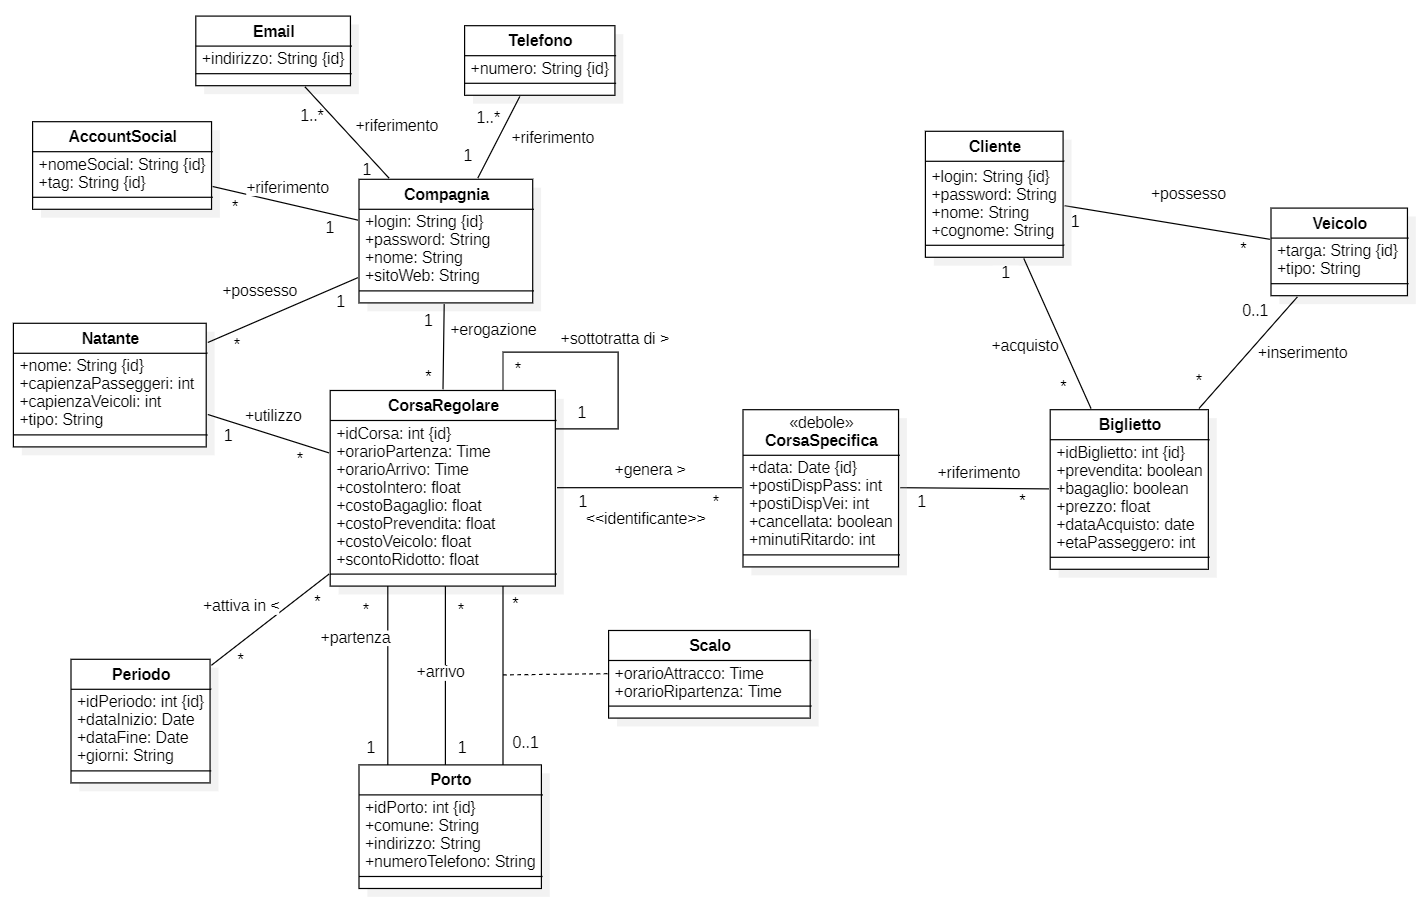
\includegraphics[width = 0.9\textwidth]{immagini/UMLdiagramRistrutturato.png}
    \label{UMLRistrutturato}
\end{figure}

\section{Traduzione al modello logico}
\subsection{Schema finale}

Gli attributi \underline{sottolineati} sono chiavi primarie, mentre gli attributi indicati con $\uparrow$ sono chiavi esterne.

\begin{table}[h!]
    \centering
    \begin{tabularx}{\textwidth}{sb} 

    \textbf{Compagnia}  &
    (\underline{login}, password, nome, sitoWeb)\\

    \textbf{CorsaRegolare}  &
    (\underline{idCorsa}, PortoPartenza$\uparrow$, PortoArrivo$\uparrow$, orarioPartenza, orarioArrivo, costoIntero, scontoRidotto, costoBagaglio, costoPrevendita, costoVeicolo, Compagnia$\uparrow$, Natante$\uparrow$, CorsaSup$\uparrow$)
    
    \textit{ PortoPartenza $\rightarrow$ Porto.idPorto}

    \textit{PortoArrivo $\rightarrow$ Porto.idPorto}

    \textit{Compagnia $\rightarrow$ Compagnia.login}

    \textit{Natante $\rightarrow$ Natante.nome} 

    \textit{CorsaSup $\rightarrow$ CorsaRegolare.idCorsa} \\

    \textbf{CorsaSpecifica}  &
    (\underline{idCorsa$\uparrow$, data}, postiDispPass, postiDispVei, minutiRitardo, cancellata)
    
    \textit{idCorsa $\rightarrow$ CorsaRegolare.idCorsa}\\

    \textbf{Periodo} &
    (\underline{idPeriodo}, datainizio, dataFine, giorni) \\

    \textbf{AttivaIn} &
    (\underline{idCorsa$\uparrow$, idPeriodo$\uparrow$}) 

    \textit{idCorsa $\rightarrow$ CorsaRegolare.idCorsa}

    \textit{idPeriodo $\rightarrow$ Periodo.idPeriodo} \\

    \textbf{Porto}  &
    (\underline{idPorto}, comune, indirizzo, numeroTelefono)\\

    \textbf{Scalo}  &
    (\underline{idCorsa$\uparrow$}, idPorto$\uparrow$, orarioAttracco, orarioRipartenza)

    \textit{idCorsa $\rightarrow$ CorsaRegolare.idCorsa}

    \textit{idPorto  $\rightarrow$ Porto.idPorto} \\

    \textbf{Natante}  &
    (\underline{nome}, capienzaPasseggeri, capienzaVeicoli, tipo, Compagnia$\uparrow$)

    \textit{Compagnia $\rightarrow$ Compagnia.login} \\

    \textbf{Cliente} & 
    (\underline{login}, password, nome, cognome) \\

    \textbf{Biglietto} &
    (\underline{idBiglietto}, idCorsa$\uparrow$, data$\uparrow$, Cliente$\uparrow$, Veicolo$\uparrow$, prevendita, bagaglio, prezzo, dataAcquisto, etaPasseggero)

        \{\textit{idCorsa},\textit{data}\}
    $\rightarrow$
         \{\textit{CorsaSpecifica.idCorsa}, \textit{CorsaSpecifica.data}\}

    \textit{Cliente $\rightarrow$ Cliente.login}

    \textit{Veicolo $\rightarrow$ Veicolo.targa} \\

    \textbf{Veicolo} &
    (\underline{targa}, tipo, Proprietario$\uparrow$)

    \textit{Proprietario $\rightarrow$ Cliente.login} \\

    \textbf{AccountSocial} &
    (\underline{nomeSocial, tag}, Compagnia$\uparrow$)

    \textit{Compagnia $\rightarrow$ Compagnia.login} \\

    \textbf{Email} &
    (\underline{indirizzo}, Compagnia$\uparrow$)

    \textit{Compagnia $\rightarrow$ Compagnia.login} \\

    \textbf{Telefono} &
    (\underline{numero}, Compagnia$\uparrow$)

    \textit{Compagnia $\rightarrow$ Compagnia.login} \\
    
    \end{tabularx}
\end{table}
\newpage

\section{Progettazione fisica}
\subsection{Creazione del database}
\begin{lstlisting}[style=sqlstyle, title = {Creazione del database}]
    --creazione di un database di nome Navigazione
    create database Navigazione;
\end{lstlisting}

\subsection{Creazione dello schema}
\begin{lstlisting}[style=sqlstyle, title = {Creazione dello schema}]
    --creazione di uno schema di nome Navigazione
    create schema Navigazione;
\end{lstlisting}

\subsection{Creazione dei tipi}
Poiché un natante può essere o un traghetto, o una motonave, o un aliscafo o nessuno di questi tre è stato scelto di definire un nuovo tipo.
\begin{lstlisting}[style=sqlstyle, title = {Creazione del tipo tipoNatante}]
    --creazione del tipo di natante come un'enumerazione dei 4 possibili tipi
    create type tipoNatante as enum ('traghetto', 'motonave', 'aliscafo', 'altro');
\end{lstlisting}

Lo stesso ragionamento è stato fatto per i tipi di veicolo che un cliente può scegliere di imbarcare.
\begin{lstlisting}[style=sqlstyle, title = {Creazione del tipo tipoVeicolo}]
    --creazione del tipo di veicolo come un'enumerazione dei 4 possibili tipi
    create type tipoVeicolo as enum ('automobile', 'motociclo', 'mezzo pesante', 'altro');
\end{lstlisting}

\subsection{Creazione delle tabelle}
La maggior parte dei vincoli di chiave esterna verranno aggiunti in un secondo momento.
\begin{lstlisting}[style=sqlstyle, title = {Creazione della tabella Compagnia}]
    create table Navigazione.Compagnia(
        login text primary key,
        password text not null,
        nome text not null,
        sitoWeb text not null
    );
\end{lstlisting}

\begin{lstlisting}[style=sqlstyle, title = {Creazione della tabella CorsaRegolare}]
    create table Navigazione.CorsaRegolare(
        idCorsa serial primary key,
        PortoPartenza integer not null,
        PortoArrivo integer not null,
        orarioPartenza time not null,
        orarioArrivo time not null,
        costoIntero numeric not null check(costoIntero >= 0),
        scontoRidotto numeric not null check(scontoRidotto >= 0 AND scontoRidotto <=100),
        costoBagaglio numeric default 0 check(costoBagaglio >= 0),
        costoPrevendita numeric default 0 check(costoPrevendita >= 0),
        costoVeicolo numeric default 0 check(costoVeicolo >= 0),
        Compagnia text not null,
        Natante text not null,
        CorsaSup integer not null,
    
        check (PortoArrivo <> PortoPartenza)
    );
\end{lstlisting}

\begin{lstlisting}[style=sqlstyle, title = {Creazione della tabella CorsaSpecifica}]
    create table Navigazione.CorsaSpecifica(
        idCorsa integer,
        data date,
        postiDispPass integer not null check(postiDispPass >= 0),
        postiDispVei integer check(postiDispVei >= 0 or postiDispVei is null),
        minutiRitardo integer not null default 0,
        cancellata boolean not null default 'false',
    
        primary key(idCorsa, data),
        foreign key(idCorsa) references Navigazione.CorsaRegolare(idCorsa)
            on delete cascade       on update cascade
    );
\end{lstlisting}

\begin{lstlisting}[style=sqlstyle, title = {Creazione della tabella Periodo}]
    create table Navigazione.Periodo(
        idPeriodo serial primary key,
        dataInizio date not null,
        dataFine date not null,
        giorni bit(7) not null,
    
        check (dataInizio < dataFine)
    );
\end{lstlisting}

\begin{lstlisting}[style=sqlstyle, title = {Creazione della tabella AttivaIn}]
    create table Navigazione.AttivaIn (
        idCorsa integer,
        idPeriodo integer,
    
        primary key(idCorsa, idPeriodo),
        foreign key(idCorsa) references Navigazione.CorsaRegolare(idCorsa)
            on delete cascade       on update cascade,
    
        foreign key(idPeriodo) references Navigazione.Periodo(idPeriodo)
            on delete cascade       on update cascade
    );
\end{lstlisting}

\begin{lstlisting}[style=sqlstyle, title = {Creazione della tabella Porto}]
    create table Navigazione.Porto(
        idPorto serial primary key,
        comune text not null,
        indirizzo text not null,
        numeroTelefono text not null
    );
\end{lstlisting}

\begin{lstlisting}[style=sqlstyle, title = {Creazione della tabella Scalo}]
    create table Navigazione.Scalo(
        idCorsa integer primary key,
        Porto integer not null,
        orarioAttracco time not null,
        orarioRipartenza time not null,
    
        check(orarioAttracco < orarioRipartenza)
    );
\end{lstlisting}

\begin{lstlisting}[style=sqlstyle, title = {Creazione della tabella Natante}]
    create table Navigazione.Natante(
        nome text primary key,
        Compagnia text not null,
        capienzaPasseggeri integer not null,
        capienzaVeicoli integer,
        tipo tipoNatante not null default 'altro'
    );
\end{lstlisting}

\begin{lstlisting}[style=sqlstyle, title = {Creazione della tabella Cliente}]
    create table Navigazione.Cliente(
        login text primary key,
        password text not null,
        nome text not null,
        cognome text not null
    );
\end{lstlisting}

\begin{lstlisting}[style=sqlstyle, title = {Creazione della tabella Biglietto}]
    create table Navigazione.Biglietto(
        idBiglietto serial primary key,
        idCorsa integer not null,
        data Date not null,
        Cliente text not null,
        Veicolo text,
        prevendita boolean not null default 'false',
        bagaglio boolean not null default 'false',
        prezzo numeric not null check(prezzo >= 0),
        dataAcquisto date not null,
        etaPasseggero integer not null check (etaPasseggero >= 0),
    
        foreign key(idCorsa, data) references Navigazione.CorsaSpecifica(idCorsa, data)
            on delete cascade       on update cascade
    );
\end{lstlisting}

\begin{lstlisting}[style=sqlstyle, title = {Creazione della tabella Veicolo}]
    create table Navigazione.Veicolo(
        targa text primary key,
        tipo tipoVeicolo not null default 'altro',
        Proprietario text not null
    );
\end{lstlisting}

\begin{lstlisting}[style=sqlstyle, title = {Creazione della tabella AccountSocial}]
    create table Navigazione.AccountSocial(
        nomeSocial text,
        tag text,
        Compagnia text not null,
    
        primary key(nomeSocial, tag)
    );
\end{lstlisting}

\begin{lstlisting}[style=sqlstyle, title = {Creazione della tabella Email}]
    create table Navigazione.Email(
        indirizzo text primary key,
        Compagnia text not null
    );
\end{lstlisting}

\begin{lstlisting}[style=sqlstyle, title = {Creazione della tabella Telefono}]
    create table Navigazione.Telefono(
        numero text primary key,
        Compagnia text not null
    );
\end{lstlisting}

\subsection{Creazione dei vincoli di chiave esterna}
\begin{lstlisting}[style=sqlstyle, title = {Aggiunti vincoli di chiave esterna per la tabella CorsaRegolare}]
    alter table Navigazione.CorsaRegolare
        add constraint corsaFKcompagnia 
            foreign key (Compagnia) references Navigazione.Compagnia(login)
                on delete cascade       on update cascade;
    
    alter table Navigazione.CorsaRegolare
        add constraint corsaFKnatante
            foreign key (Natante) references Navigazione.Natante(nome)
                on delete cascade   on update cascade;
    
    alter table Navigazione.CorsaRegolare
        add constraint corsaFKportoPartenza
            foreign key (PortoPartenza) references Navigazione.Porto(idPorto)
                on delete cascade       on update cascade;
    
    alter table Navigazione.CorsaRegolare
        add constraint corsaFKportoArrivo
            foreign key (PortoArrivo) references Navigazione.Porto(idPorto)
                on delete cascade       on update cascade;
    
    alter table Navigazione.CorsaRegolare
        add constraint corsaFKcorsaSup
            foreign key (CorsaSup) references Navigazione.CorsaRegolare(idCorsa)
                on delete cascade       on update cascade;
\end{lstlisting}

\begin{lstlisting}[style=sqlstyle, title = {Aggiunti vincoli di chiave esterna per la tabella Scalo}]
    alter table Navigazione.Scalo
        add constraint scaloFKcorsa
            foreign key (idCorsa) references Navigazione.CorsaRegolare(idCorsa)
                on delete cascade       on update cascade;
    
    alter table Navigazione.Scalo
        add constraint scaloFKporto
            foreign key (Porto) references Navigazione.Porto(idPorto)
                on delete cascade       on update cascade;
\end{lstlisting}

\begin{lstlisting}[style=sqlstyle, title = {Aggiunto vincolo di chiave esterna per la tabella Natante}]
    alter table Navigazione.Natante
        add constraint natanteFKcompagnia
            foreign key (Compagnia) references Navigazione.Compagnia(login)
                on delete cascade       on update cascade;
\end{lstlisting}

\begin{lstlisting}[style=sqlstyle, title = {Aggiunti vincoli di chiave esterna per la tabella Biglietto}]
    alter table Navigazione.Biglietto
        add constraint bigliettoFKcliente
            foreign key (Cliente) references Navigazione.Cliente(login)
                on delete cascade       on update cascade;
    
    alter table Navigazione.Biglietto
        add constraint bigliettoFKveicolo
            foreign key (Veicolo) references Navigazione.Veicolo(targa)
                on delete set null      on update cascade;
\end{lstlisting}

\begin{lstlisting}[style=sqlstyle, title = {Aggiunto vincolo di chiave esterna per la tabella Veicolo}]
    alter table Navigazione.Veicolo
        add constraint veicoloFKproprietario
            foreign key (Proprietario) references Navigazione.Cliente(login)
                on delete cascade       on update cascade;
\end{lstlisting}

\begin{lstlisting}[style=sqlstyle, title = {Aggiunto vincolo di chiave esterna per la tabella AccountSocial}]
    alter table Navigazione.AccountSocial
        add constraint accountFKcompagnia
            foreign key (Compagnia) references Navigazione.Compagnia(login)
                on delete cascade       on update cascade;
\end{lstlisting}

\begin{lstlisting}[style=sqlstyle, title = {Aggiunto vincolo di chiave esterna per la tabella Email}]
    alter table Navigazione.Email
        add constraint emailFKcompagnia
            foreign key (Compagnia) references Navigazione.Compagnia(login)
                on delete cascade       on update cascade;
\end{lstlisting}

\begin{lstlisting}[style=sqlstyle, title = {Aggiunto vincolo di chiave esterna per la tabella Telefono}]
    alter table Navigazione.Telefono
        add constraint telefonoFKcompagnia
            foreign key (Compagnia) references Navigazione.Compagnia(login)
                on delete cascade       on update cascade;
\end{lstlisting}

\subsection{Trigger e trigger function}
\label{sec:ImplementazioneTrigger}
La descrizione dei trigger è riportata nella sezione \hyperref[sec:VincoliInterRelazionali]{Vincoli Inter-Relazionali}.

\begin{lstlisting}[style=sqlstyle]
-- trigger per aggiornare i posti (per passeggeri) disponibili per una corsa specifica
create function aggiornapostipasseggero() returns trigger
    language plpgsql
as
$$
declare
    v_corsa_sup navigazione.corsaregolare.corsasup%type;
begin
    select corsasup into v_corsa_sup
    from navigazione.corsaregolare
    where idcorsa = new.idcorsa;

    raise notice 'corsa sup %', v_corsa_sup;
    --se il biglietto acquistato e' per una corsa principale 
    if v_corsa_sup is null then 
        --aggiorna i posti disponibili anche per le sottocorse
        update navigazione.corsaspecifica
        set postidisppass = postidisppass - 1
        where data = new.data and idcorsa in (select CR.idcorsa
                                              from navigazione.corsaregolare as CR
                                              where CR.corsasup = new.idcorsa or CR.idcorsa = new.idcorsa);
    else --se invece il biglietto acquistato e' per una sottotratta 
        --aggiorna i posti per la sottotratta in questione
        update navigazione.corsaspecifica
        set postidisppass = postidisppass - 1
        where idcorsa = new.idCorsa and data = new.data;
        
        --aggiorna i posti per la corsa principale
        update navigazione.corsaspecifica
        set postidisppass = postidisppass - 1
        where idcorsa = v_corsa_sup and data = new.data;
    end if;
    
    return null;
end;
$$;
----------
create trigger triggeraggiornapostipasseggero
    after insert
    on biglietto
    for each row
execute procedure aggiornapostipasseggero();
\end{lstlisting}

\begin{lstlisting}[style = sqlstyle]
-- trigger per aggiornare i posti (per veicoli) disponibili per una corsa specifica
create function aggiornapostiveicolo() returns trigger
    language plpgsql
as
$$
declare
    v_corsa_sup navigazione.corsaregolare.corsasup%type;
begin
    select corsasup into v_corsa_sup
    from navigazione.corsaregolare
    where idcorsa = new.idcorsa;

    --se il biglietto acquistato e' per una corsa principale 
    if v_corsa_sup is null then
        --aggiorna i posti disponibili anche per le sottocorse
        update navigazione.corsaspecifica
        set postidispvei = postidispvei - 1
        where data = new.data and idcorsa in (select CR.idcorsa
                                              from navigazione.corsaregolare as CR
                                              where CR.corsasup = new.idcorsa or CR.idcorsa = new.idcorsa);
    else --se invece il biglietto acquistato e' per una sottotratta 
        --aggiorna i posti per la sottotratta in questione
        update navigazione.corsaspecifica
        set postidispvei = postidispvei - 1
        where idcorsa = new.idCorsa and data = new.data;

        --aggiorna i posti per la corsa principale
        update navigazione.corsaspecifica
        set postidispvei = postidispvei - 1
        where idcorsa = v_corsa_sup and data = new.data;
    end if;

    return null;
end;
$$;
----------
create trigger triggeraggiornapostiveicolo
    after insert
    on biglietto
    for each row
    when (new.veicolo IS NOT NULL)
execute procedure aggiornapostiveicolo();
\end{lstlisting}

\begin{lstlisting}[style = sqlstyle]
-- all'inserimento di uno scalo per una corsaregolare, questo trigger si occupa di generare le sottocorse e di attivarle nei periodi
--in cui e' attiva la corsa principale.
create function aggiungicorsescalo() returns trigger
    language plpgsql
as
$$
declare
    v_record navigazione.corsaregolare%rowtype;
    v_ultimo_idcorsa navigazione.corsaregolare.idcorsa%type;
    --seleziona tutti i periodi in cui e' attiva la corsa principale
    cur_periodi cursor for
        select idperiodo
        from navigazione.attivain
        where idcorsa = new.idcorsa;
begin
    --seleziona in corsaRegolare l'intera tupla corrispondente alla corsa principale
    select * into v_record
    from navigazione.corsaregolare
    where idcorsa = new.idcorsa;

    --inserisce in corsaRegolare la prima sottotratta che parte dal porto di partenza della corsa principale
    --e arriva al porto di scalo
    insert into navigazione.corsaregolare(portopartenza, portoarrivo, orariopartenza, orarioarrivo,
                                          costointero, scontoridotto, costobagaglio, costoprevendita,
                                          costoveicolo, compagnia, natante, corsasup)
    values
        (v_record.portopartenza, new.porto, v_record.orariopartenza, new.orarioAttracco, v_record.costointero,
         v_record.scontoridotto, v_record.costobagaglio, v_record.costoprevendita, v_record.costoveicolo,
         v_record.compagnia, v_record.natante, new.idcorsa);

    --seleziona quest'ultima corsa inserita
    select idcorsa into v_ultimo_idcorsa
    from navigazione.corsaregolare
    order by idcorsa desc
    limit 1;

    --e l'attiva in tutti i periodi in cui era attiva la corsa principale
    for p in cur_periodi loop
        insert into navigazione.attivain
        values (v_ultimo_idcorsa, p.idperiodo);
    end loop;

    --inserisce in corsaRegolare la seconda sottotratta che parte dal porto di scalo 
    --e arriva al porto di arrivo della corsa principale
    insert into navigazione.corsaregolare(portopartenza, portoarrivo, orariopartenza, orarioarrivo,
                                          costointero, scontoridotto, costobagaglio, costoprevendita,
                                          costoveicolo, compagnia, natante, corsasup)
    values
        (new.porto, v_record.portoarrivo, new.orarioRipartenza, v_record.orarioarrivo, v_record.costointero,
         v_record.scontoridotto, v_record.costobagaglio, v_record.costoprevendita, v_record.costoveicolo,
         v_record.compagnia, v_record.natante, new.idcorsa);

    --seleziona quest'ultima corsa inserita
    select idcorsa into v_ultimo_idcorsa
    from navigazione.corsaregolare
    order by idcorsa desc
    limit 1;

    --e l'attiva in tutti i periodi in cui era attiva la corsa principale
    for p in cur_periodi loop
            insert into navigazione.attivain
            values (v_ultimo_idcorsa, p.idperiodo);
    end loop;
    
    return new;
end;
$$;
----------
create trigger generatrattescalotrigger
    after insert
    on scalo
    for each row
execute procedure aggiungicorsescalo();
\end{lstlisting}

\begin{lstlisting}[style = sqlstyle]
-- trigger per attivare nei periodi della corsa principale anche le sue sottocorse
create function attivasottocorse() returns trigger
    language plpgsql
as
$$
declare
    --seleziona le due sottocorse della corsa in questione
    cur_sottocorse cursor for
        select idcorsa
        from navigazione.corsaregolare
        where corsasup = new.idcorsa;
begin
    --e attiva ognuna nel nuovo periodo inserito
    for t in cur_sottocorse loop
        insert into navigazione.attivain
        values (t.idcorsa, new.idperiodo);
    end loop;

    return new;
end;
$$;
----------
create trigger attivasottocorsetrigger
    after insert
    on attivain
    for each row
execute procedure attivasottocorse();
\end{lstlisting}

\begin{lstlisting}[style=sqlstyle]
--trigger che quando viene cambiato l'orario di arrivo della corsa principale
--aggiorna l'orario di arrivo anche della sottocorsa che parte dal porto di scalo
create function cambiaorarioarrivoinsottocorsa() returns trigger
    language plpgsql
as
$$
declare
    sottocorsa navigazione.corsaregolare%rowtype;
begin
    --seleziona la sottocorsa che arriva allo stesso orario della corsa principale
    select * into sottocorsa
    from navigazione.corsaregolare
    where corsasup = old.idcorsa and orarioarrivo = old.orarioarrivo;

    --aggiorna l'orario di arrivo
    update navigazione.corsaregolare
    set orarioarrivo = new.orarioarrivo
    where idcorsa = sottocorsa.idcorsa;

    return new;
end;
$$;
----------
create trigger cambiaorarioarrivoinsottocorsa
    after update
        of orarioarrivo
    on corsaregolare
    for each row
    --quando e' una corsa principale
    when (new.corsasup IS NULL AND new.orarioarrivo IS NOT NULL)
execute procedure cambiaorarioarrivoinsottocorsa();

\end{lstlisting}

\begin{lstlisting}[style=sqlstyle]
--trigger che quando viene cambiato l'orario di partenza della corsa principale
--aggiorna l'orario di partenza anche della sottocorsa che parte dallo stesso porto
create function cambiaorariopartenzainsottocorsa() returns trigger
    language plpgsql
as
$$
declare
    sottocorsa navigazione.corsaregolare%rowtype;

begin
    --seleziona la sottocorsa che parte allo stesso orario della corsa principale
    select * into sottocorsa
    from navigazione.corsaregolare
    where corsasup = old.idcorsa and orariopartenza = old.orariopartenza;

    --aggiorna l'orario di partenza
    update navigazione.corsaregolare
    set orariopartenza = new.orariopartenza
    where idcorsa = sottocorsa.idcorsa;

    return new;
end;
$$;
----------
create trigger cambiaorariopartenzainsottocorsa
    after update
        of orariopartenza
    on corsaregolare
    for each row
    when (new.corsasup IS NULL AND new.orariopartenza IS NOT NULL)
execute procedure cambiaorariopartenzainsottocorsa();

\end{lstlisting}

\begin{lstlisting}[style=sqlstyle]
--trigger per eliminare le corse specifiche di una corsa regolare non piu' attiva in un periodo
--ed eliminare i periodi che non sono attaccati a nessuna corsa
create function cancellacorseinperiodo() returns trigger
    language plpgsql
as
$$
declare
    v_data_inizio navigazione.periodo.datainizio%type;
    v_data_fine navigazione.periodo.dataFine%type;
    v_data_corrente date;
    v_giorni bit(7);
    v_day integer;
    v_offset integer;
    --trovo i periodi che non sono attaccati a nessuna corsa
    cur_periodi cursor for
        select P.idperiodo
        from navigazione.periodo as P
        where P.idperiodo not in (select idperiodo 
                                  from navigazione.attivain);
begin
    select datainizio, datafine, giorni into v_data_inizio, v_data_fine, v_giorni
    from navigazione.periodo
    where idperiodo = old.idperiodo;

    --ricava un numero da 0 a 6 corrispondente al giorno della settimana in cui inizia il periodo
    -- 0 se domenica, 1 se lunedi' ... fino a 6 se sabato
    v_day := extract(dow from v_data_inizio::timestamp);
    --per ogni bit della stringa di bit che indica i giorni di attivita'
    for i in 0..6 loop
        --ogni iterazione del for-loop parte con v_data_corrente uguale alla data di inizio
        v_data_corrente := v_data_inizio;
        --se l'i-esimo bit e' 1
        if get_bit(v_giorni, i) = 1 then
            v_offset := (i - v_day);
            if v_offset < 0 then
                while v_offset < 0 loop
                        v_offset := v_offset + 7;
                end loop;
            else
                v_offset := v_offset % 7;
            end if;
            --aggiunge l'offset alla data corrente affinche' la data corrente
            --si trovi nella prima data maggiore o uguale la data di inizio,
            --che abbia come giorno della settimana l'i-esimo giorno
            v_data_corrente := v_data_corrente + v_offset;
            --per tutte le date con quel giorno incluse nel periodo
            while v_data_corrente <= v_data_fine loop
                --elimina la corsa specifica per quella data
                delete from navigazione.corsaspecifica
                where idcorsa = old.idcorsa AND data = v_data_corrente;
                --incrementa la data alla settimana successiva
                v_data_corrente := v_data_corrente + 7;
            end loop;
        end if;
    end loop;

    --elimina i periodi che non sono attaccati a nessuna corsa
    for p in cur_periodi loop
        delete from navigazione.periodo
        where idperiodo = p.idperiodo;
    end loop;
    
    return null;
end;
$$;
----------
create trigger cancellacorse
    after delete
    on attivain
    for each row
execute procedure cancellacorseinperiodo();

\end{lstlisting}

\begin{lstlisting}[style = sqlstyle]
--Trigger per eliminare le sottocorse dopo che e' stato eliminato uno scalo
create function eliminacorsescalo() returns trigger
    language plpgsql
as
$$
begin
    delete from navigazione.corsaregolare
    where corsasup = old.idcorsa AND (portopartenza = old.porto OR portoarrivo = old.porto);
    
    return null;
end;
$$;
----------
create trigger eliminatrattescalotrigger
    after delete
    on scalo
    for each row
execute procedure eliminacorsescalo();

\end{lstlisting}

\begin{lstlisting}[style = sqlstyle]
--Trigger per eliminare l'altra sottocorsa dopo che ne e' stata eliminata una, poiche' non puo' esistere una senza l'altra. 
create function eliminasottocorse() returns trigger
    language plpgsql
as
$$
declare
    v_altra_corsa navigazione.corsaregolare.idcorsa%type;
begin
    if old.corsasup is not null then
        --seleziona la sottocorsa rimanente
        select idcorsa into v_altra_corsa
        from navigazione.corsaregolare
        where corsasup = old.corsasup;

        if v_altra_corsa is not null then
            --e la cancella
            delete from navigazione.corsaregolare
            where idcorsa = v_altra_corsa;
        end if;
        
        --elimina la tupla in scalo che aveva generato le due sottocorse
        delete from navigazione.scalo
        where idcorsa = old.corsasup;
    end if;
    return null;
end;
$$;
----------
create trigger eliminaaltrasottocorsa
    after delete
    on corsaregolare
    for each row
    --quando la corsa eliminata e' una sottocorsa
    when (old.corsasup IS NOT NULL)
execute procedure eliminasottocorse();

\end{lstlisting}

\begin{lstlisting}[style=sqlstyle]
-- trigger per la generazione delle corse specifiche in tutte le date presenti nel periodo di attivazione
create function generacorsespecifiche() returns trigger
    language plpgsql
as
$$
declare
    v_data_inizio date;
    v_data_corrente date;
    v_data_fine date;
    v_giorni bit(7);
    v_natante navigazione.natante.nome%type;
    v_cap_pass integer;
    v_cap_veic integer;
    v_day integer;
    v_offset integer;
begin
    --seleziona le date di inizio e fine e i giorni del periodo
    select dataInizio, dataFine, giorni into v_data_inizio, v_data_fine, v_giorni
    from navigazione.periodo
    where idperiodo = new.idperiodo;

    --seleziona il natante che verra' utilizzato
    select natante into v_natante
    from navigazione.corsaRegolare
    where idcorsa = new.idcorsa;

    --seleziona la capienza passeggeri e veicoli del natante
    select capienzaPasseggeri, capienzaVeicoli into v_cap_pass, v_cap_veic
    from navigazione.natante
    where nome = v_natante;

    --ricava un numero da 0 a 6 corrispondente al giorno della settimana in cui inizia il periodo
    -- 0 se domenica, 1 se lunedi' ... fino a 6 se sabato
    v_day := extract(dow from v_data_inizio::timestamp);
    --per ogni bit della stringa di bit che indica i giorni di attivita'
    for i in 0..6 loop
        --ogni iterazione del for-loop parte con v_data_corrente uguale alla data di inizio
        v_data_corrente := v_data_inizio;
        --se l'i-esimo bit e' 1
        if get_bit(v_giorni, i) = 1 then
            v_offset := (i - v_day);
            if v_offset < 0 then
                while v_offset < 0 loop
                    v_offset := v_offset + 7;
                end loop;
            else
                v_offset := v_offset % 7;
            end if;
            --aggiunge l'offset alla data corrente affinche' la data corrente
            --si trovi nella prima data maggiore o uguale la data di inizio,
            --che abbia come giorno della settimana l'i-esimo giorno
            v_data_corrente := v_data_corrente + v_offset;
            --per tutte le date con quel giorno incluse nel periodo
            while v_data_corrente <= v_data_fine loop
                --aggiunge la corsa specifica per quella data
                insert into navigazione.corsaSpecifica
                values(new.idcorsa, v_data_corrente, v_cap_pass, v_cap_veic, 0, false);
                --incrementa la data alla settimana successiva
                v_data_corrente := v_data_corrente + 7;
            end loop;
        end if;
    end loop;
    
    return new;
end;
$$;
----------
create trigger generacorse
    after insert
    on attivain
    for each row
execute procedure generacorsespecifiche();

\end{lstlisting}

\begin{lstlisting}[style=sqlstyle]
-- trigger per cancellare le sottocorse figlie (quando viene cancellata una corsa principale), e la
-- sottocorsa sorella (quando viene cancellata una sottocorsa).
create function propagacancellazione() returns trigger
    language plpgsql
as
$$
declare
    thisData date := old.data;
    CorsaRegolareRiferita navigazione.corsaregolare%rowtype;
    isCancellata boolean;
    it1 cursor for select *
                   from  navigazione.corsaregolare
                   where corsasup = CorsaRegolareRiferita.idcorsa;
    it2 cursor for select *
                    from navigazione.corsaregolare
                    where corsasup = CorsaRegolareRiferita.corsasup and idcorsa <> CorsaRegolareRiferita.idcorsa;
begin
    --seleziona la corsa regolare della corsa in questione
    select * into CorsaRegolareRiferita from navigazione.corsaregolare where idcorsa = old.idcorsa;
    --se e' una corsa principale
    if (CorsaRegolareRiferita.corsasup is null) then --potrebbe avere delle sottocorse
        --per entrambe le sottocorse
        for x in it1 loop
            select cancellata into isCancellata
            from navigazione.corsaspecifica
            where idcorsa = x.idcorsa and data = thisData;
            --se non sono gia' cancellate le cancella
            if isCancellata = false then
                update navigazione.corsaspecifica
                set cancellata = true
                where idcorsa = x.idcorsa and data = thisData;
            end if;
        end loop;
    else --se invece e' una sottocorsa ha sicuramente una sorella
        for x in it2 loop
            --e cancella entrambe
            select cancellata into isCancellata
            from navigazione.corsaspecifica
            where idcorsa = x.idcorsa and data = thisData;
            if isCancellata = false then
                update navigazione.corsaspecifica
                set cancellata = true
                where idcorsa = x.idcorsa and data = thisData;
            end if;
        end loop;
    end if;
    return new;
end;
$$;
----------
create trigger propagacancellazione
    after update
        of cancellata
    on corsaspecifica
    for each row
    when (new.cancellata = true)
execute procedure propagacancellazione();
\end{lstlisting}

\subsection{Procedure}
\begin{lstlisting}[style=sqlstyle]
--Procedura per calcolare gli incassi di una corsa regolare in un determinato arco di tempo
create procedure calcolaincassicorsainperiodo(IN thisidcorsa integer, IN ini_periodo date, IN fin_periodo date, OUT incasso double precision)
    language plpgsql
as
$$
begin
    select sum(prezzo) into incasso
    from navigazione.biglietto
    where idcorsa = thisidcorsa and data between ini_periodo and fin_periodo;
end;
$$;

\end{lstlisting}

\begin{lstlisting}[style=sqlstyle]
--Procedura per fare in modo che quando venga creato uno scalo in una corsa regolare, per ogni data
--in cui e' attiva, le sottocorse create abbiano gli stessi posti disponibili della corsa madre.
create procedure aggiornapostisottocorse(IN idcorsa_in integer)
    language plpgsql
as
$$
declare
    --seleziona le sottocorse
    cur_sottocorse cursor for
        select CR.idcorsa
        from navigazione.corsaregolare as CR
        where CR.corsasup = idCorsa_in;

    --seleziona i dati che vanno aggiornati nelle sottocorse
    cur_postidisp cursor for
        select CS.idcorsa, CS.data, CS.postidisppass, CS.postidispvei, CS.cancellata
        from navigazione.corsaspecifica as CS
        where CS.idcorsa = idCorsa_in;
begin
    for k in cur_postidisp loop
        for i in cur_sottocorse loop
            --aggiorna i valori delle sottocorse
            update navigazione.corsaspecifica
            set postidisppass = k.postidisppass, postidispvei = k.postidispvei, cancellata = k.cancellata
            where idcorsa = i.idcorsa AND data = k.data;
        end loop;
    end loop;
end;
$$;
\end{lstlisting}
\newpage

\subsection{Dizionario dei vincoli}
\subsubsection{Vincoli Intra-Relazionali}

\begin{longtable}{|| m{0.3\textwidth} | m{0.7\textwidth} ||}
    \hline\hline
     \textbf{Vincolo} & \textbf{Descrizione} \\ [1ex]
     \hline\hline
     \endfirsthead

      \textit{accountsocial\_pkey} & Vincolo di chiave primaria  \\ [1ex]
      \hline

      \textit{accountfkcompagnia} & Vincolo di chiave esterna. Se viene eliminata la compagnia vengono eliminati anche tutti i suoi account social. \\ [1ex]
     \hline\hline

     \caption*{Tabella AccountSocial} \\
\end{longtable}

\begin{longtable}{|| m{0.4\textwidth} | m{0.6\textwidth} ||}
    \hline\hline
     \textbf{Vincolo} & \textbf{Descrizione} \\ [1ex]
     \hline\hline
     \endfirsthead

      \textit{attivain\_pkey} & Vincolo di chiave primaria  \\ [1ex]
      \hline

      \textit{attivain\_idcorsa\_fkey} & Vincolo di chiave esterna. Se viene eliminata la corsa regolare vengono eliminate anche le tuple associate in AttivaIn. \\ [1ex]
     \hline

     \textit{attivain\_idperiodo\_fkey} & Vincolo di chiave esterna. Se viene eliminato un periodo vengono eliminate anche le tuple associate in AttivaIn. \\ [1ex]
     \hline\hline

     \caption*{Tabella AttivaIn} \\
\end{longtable}

\begin{longtable}{|| m{0.4\textwidth} | m{0.6\textwidth} ||}
    \hline\hline
     \textbf{Vincolo} & \textbf{Descrizione} \\ [1ex]
     \hline\hline
     \endfirsthead

      \textit{biglietto\_pkey} & Vincolo di chiave primaria  \\ [1ex]
      \hline

      \textit{biglietto\_idcorsa\_data\_fkey} & Vincolo di chiave esterna. Se viene eliminata una corsa specifica anche i biglietti associati verranno eliminati \\ [1ex]
     \hline

     \textit{bigliettofkcliente} & Vincolo di chiave esterna. Se viene eliminato un cliente anche i biglietti associati verrano eliminati \\ [1ex]
     \hline

     \textit{bigliettofkveicolo} & Vincolo di chiave esterna. Se viene eliminato un veicolo il valore in biglietto sarà settato a null \\ [1ex]
     \hline

     \textit{biglietto\_etapasseggero\_check} & Controlla che l'età del passeggero sia un numero non negativo. \\ [1ex]
     \hline

     \textit{biglietto\_prezzo\_check} & Controlla che il prezzo del biglietto sia un numero non negativo. \\ [1ex]
     \hline\hline

     \caption*{Tabella Biglietto} \\
\end{longtable}

\begin{longtable}{|| m{0.3\textwidth} | m{0.7\textwidth} ||}
    \hline\hline
     \textbf{Vincolo} & \textbf{Descrizione} \\ [1ex]
     \hline\hline
     \endfirsthead

      \textit{cliente\_pkey} & Vincolo di chiave primaria. \\ [1ex]
     \hline\hline

     \caption*{Tabella Cliente} \\
\end{longtable}

\begin{longtable}{|| m{0.3\textwidth} | m{0.7\textwidth} ||}
    \hline\hline
     \textbf{Vincolo} & \textbf{Descrizione} \\ [1ex]
     \hline\hline
     \endfirsthead

      \textit{compagnia\_pkey} & Vincolo di chiave primaria. \\ [1ex]
     \hline\hline

     \caption*{Tabella Compagnia} \\
\end{longtable}

\begin{longtable}{|| m{0.5\textwidth} | m{0.5\textwidth} ||}
    \hline\hline
     \textbf{Vincolo} & \textbf{Descrizione} \\ [1ex]
     \hline\hline
     \endfirsthead

      \textit{corsaregolare\_pkey} & Vincolo di chiave primaria. \\ [1ex]
        \hline

      \textit{corsafkcompagnia} & Vincolo di chiave esterna. Se viene eliminata la compagnia verrano eliminati anche tutte le sue corse regolari. \\ [1ex]
     \hline

     \textit{corsafkcorsasup} & Vincolo di chiave esterna. Se viene eliminata la corsa principale anche le sottocorse verranno eliminate. \\ [1ex]
     \hline

     \textit{corsafkportoarrivo} & Vincolo di chiave esterna. Se viene eliminato il porto di arrivo, verranno eliminate tutte le corse che arrivano in quel porto. \\ [1ex]
     \hline

     \textit{corsafkportopartenza} & Vincolo di chiave esterna. Se viene eliminato il porto di partenza, verranno eliminate tutte le corse che partivano da quel porto. \\ [1ex]
     \hline

    \textit{corsafknatante} & Vincolo di chiave esterna. Se viene eliminato il natante, verrano eliminate tutte le corse che usavano quel natante. \\ [1ex]
     \hline

     \textit{corsaregolare\_check} & Controlla che il porto di arrivo sia diverso dal porto di partenza. \\ [1ex]
     \hline

     \textit{corsaregolare\_costobagaglio\_check} & Controlla che il costo del bagaglio sia un numero non negativo. \\ [1ex]
     \hline

     \textit{corsaregolare\_costointero\_check} & Controlla che il costo intero della corsa sia un numero non negativo. \\ [1ex]
     \hline

     \textit{corsaregolare\_costoprevendita\_check} & Controlla che il costo della prevendita sia un numero non negativo. \\ [1ex]
     \hline

     \textit{corsaregolare\_costoveicolo\_check} & Controlla che il costo del veicolo sia un numero non negativo. \\ [1ex]
     \hline

     \textit{corsaregolare\_scontoridotto\_check} & Controlla che la percentuale di sconto sia un numero compreso tra $0$ e $100$. \\ [1ex]      
     \hline\hline

     \caption*{Tabella CorsaRegolare} \\
\end{longtable}

\begin{longtable}{|| m{0.5\textwidth} | m{0.5\textwidth} ||}
    \hline\hline
     \textbf{Vincolo} & \textbf{Descrizione} \\ [1ex]
     \hline\hline
     \endfirsthead

      \textit{corsaspecifica\_pkey} & Vincolo di chiave primaria. \\ [1ex]
      \hline

      \textit{corsaspecifica\_idcorsa\_fkey} & Vincolo di chiave esterna. Se viene eliminata una corsa regolare, tutte le corse specifiche associato verranno eliminate. \\ [1ex]
      \hline
        
      \textit{corsaspecifica\_postidisppass\_check} & Controlla che i posti passeggeri disponibili sia un numero non negativo \\ [1ex]
     \hline

     \textit{corsaspecifica\_postidisppass\_check} & Controlla che i posti veicoli disponibili siano un numero non negativo \\ [1ex]      
     \hline\hline

     \caption*{Tabella CorsaSpecifica} \\
\end{longtable}
\newpage

\begin{longtable}{|| m{0.3\textwidth} | m{0.7\textwidth} ||}
    \hline\hline
     \textbf{Vincolo} & \textbf{Descrizione} \\ [1ex]
     \hline\hline
     \endfirsthead

      \textit{email\_pkey} & Vincolo di chiave primaria. \\ [1ex]
      \hline

      \textit{emailfkcompagnia} & Vincolo di chiave esterna. Se una compagnia viene eliminata anche tutte le sue email verrano eliminate. \\ [1ex]      
     \hline\hline

     \caption*{Tabella Email} \\
\end{longtable}

\begin{longtable}{|| m{0.3\textwidth} | m{0.7\textwidth} ||}
    \hline\hline
     \textbf{Vincolo} & \textbf{Descrizione} \\ [1ex]
     \hline\hline
     \endfirsthead

      \textit{natante\_pkey} & Vincolo di chiave primaria. \\ [1ex]
      \hline

      \textit{natantefkcompagnia} & Vincolo di chiave esterna. Se una compagnia viene eliminata anche i natanti da essa posseduta verranno eliminati. \\ [1ex]      
     \hline\hline

     \caption*{Tabella Natante} \\
\end{longtable}

\begin{longtable}{|| m{0.3\textwidth} | m{0.7\textwidth} ||}
    \hline\hline
     \textbf{Vincolo} & \textbf{Descrizione} \\ [1ex]
     \hline\hline
     \endfirsthead

      \textit{periodo\_pkey} & Vincolo di chiave primaria. \\ [1ex]
      \hline

      \textit{periodo\_check} & Controlla che la data di inizio periodo sia minore o uguale alla data di fine periodo. \\ [1ex]      
     \hline\hline

     \caption*{Tabella Periodo} \\
\end{longtable}

\begin{longtable}{|| m{0.3\textwidth} | m{0.7\textwidth} ||}
    \hline\hline
     \textbf{Vincolo} & \textbf{Descrizione} \\ [1ex]
     \hline\hline
     \endfirsthead

      \textit{porto\_pkey} & Vincolo di chiave primaria. \\ [1ex]    
     \hline\hline

     \caption*{Tabella Porto} \\
\end{longtable}

\begin{longtable}{|| m{0.3\textwidth} | m{0.7\textwidth} ||}
    \hline\hline
     \textbf{Vincolo} & \textbf{Descrizione} \\ [1ex]
     \hline\hline
     \endfirsthead

      \textit{scalo\_pkey} & Vincolo di chiave primaria. \\ [1ex]
      \hline

      \textit{scalofkcorsa} & Vincolo di chiave esterna. Se una corsa viene eliminata, anche lo scalo associato viene eliminato. \\ [1ex]
      \hline

      \textit{scalofkporto} & Vincolo di chiave esterna. Se un porto viene eliminato, anche gli scali in quel porto verranno eliminati. \\ [1ex]
      \hline

      \textit{scalo\_check} & Controlla che l'orario di attracco sia minore dell'orario di ripartenza. \\ [1ex]     
     \hline\hline

     \caption*{Tabella Scalo} \\
\end{longtable}

\begin{longtable}{|| m{0.3\textwidth} | m{0.7\textwidth} ||}
    \hline\hline
     \textbf{Vincolo} & \textbf{Descrizione} \\ [1ex]
     \hline\hline
     \endfirsthead

      \textit{telefono\_pkey} & Vincolo di chiave primaria. \\ [1ex]
      \hline

      \textit{telefonofkcompagnia} & Vincolo di chiave esterna. Se una compagnia viene eliminata anche i suoi numeri telefonici verranno eliminati.\\ [1ex]      
     \hline\hline

     \caption*{Tabella Telefono} \\
\end{longtable}

\begin{longtable}{|| m{0.3\textwidth} | m{0.7\textwidth} ||}
    \hline\hline
     \textbf{Vincolo} & \textbf{Descrizione} \\ [1ex]
     \hline\hline
     \endfirsthead

      \textit{veicolo\_pkey} & Vincolo di chiave primaria. \\ [1ex]
      \hline

      \textit{veicolofkproprietario} & Vincolo di chiave esterna. Se un cliente viene eliminato anche tutti i suoi veicoli verranno eliminati.\\ [1ex]      
     \hline\hline

     \caption*{Tabella Veicolo} \\
\end{longtable}

\subsubsection{Vincoli Inter-Relazionali}
\label{sec:VincoliInterRelazionali}

L'implementazione dei trigger è riportata nella sezione \hyperref[sec:ImplementazioneTrigger]{Trigger e trigger function}.

\begin{longtable}{|| m{0.45\textwidth} | m{0.55\textwidth} ||}
    \hline\hline
     \textbf{Trigger} & \textbf{Descrizione} \\ [1ex]
     \hline\hline
     \endfirsthead

      \textit{attivaSottoCorseTrigger} & Dopo aver inserito una tupla in \textit{AttivaIn}, anche le eventuali sottocorse della corsa inserita verranno inserite in \textit{AttivaIn}. \\ [1ex]
      \hline

      \textit{cancellaCorseTrigger} & Dopo aver eliminato una una tupla in \textit{AttivaIn}, vengono eliminate tutte le corse specifiche relative a quella corsa, in tutte le date appartenenti a quel periodo \\ [1ex]
      \hline

      \textit{generaCorse} & Dopo aver inserito una tupla in \textit{AttivaIn}, per tutte le date appartenti al periodo in questione verranno inserite delle corse specifiche. \\ [1ex]
      \hline

      \textit{triggerAggiornaPostiPasseggero} & Dopo aver inserito una tupla in \textit{Biglietto}, il trigger aggiorna i posti disponibili per quella corsa specifica, inoltre se la corsa in questione è una corsa principale, il trigger aggiornerà i posti anche per le sottocorse, se invece la corsa è una sottocorsa, il trigger aggionerà i posti anche per la corsa principale ma non per l'altra sottocorsa. \\ [1ex]
      \hline

      \textit{triggerAggiornaPostiVeicolo} & Dopo aver inserito una tupla in \textit{Biglietto}, il trigger aggiorna i posti disponibili per quella corsa specifica, inoltre se la corsa in questione è una corsa principale, il trigger aggiornerà i posti anche per le sottocorse, se invece la corsa è una sottocorsa, il trigger aggionerà i posti anche per la corsa principale ma non per l'altra sottocorsa. Il trigger si attiva solo quando il valore di \textit{veicolo} è diverso da null. \\ [1ex]
      \hline

      \textit{cambiaOrarioArrivoInSottocorsa} & Dopo aver modificato il valore di \textit{orarioArrivo} in \textit{CorsaRegolare}, il trigger modificherà il valore anche nelle eventuali sottocorse. Il trigger si attiva quindi solo quando \textit{corsaSup} è null. \\ [1ex]
      \hline

      \textit{cambiaOrarioPartenzaInSottocorsa} & Dopo aver modificato il valore di \textit{orarioPartenza} in \textit{CorsaRegolare}, il trigger modificherà il valore anche nelle eventuali sottocorse. Il trigger si attiva quindi solo quando \textit{corsaSup} è null. \\ [1ex]
      \hline

      \textit{eliminaAltraSottocorsa} & Dopo aver eliminato una tupla in \textit{CorsaRegolare} e quando \textit{corsaSup} è diverso da null, quindi si è appena eliminata una sottocorsa, il trigger andrà ad eliminare anche l'altra sottocorsa che ha lo stesso valore di \textit{corsaSup}. \\ [1ex]
      \hline

      \textit{propagaCancellazione} & Dopo aver settato a \textit{true} il valore di \textit{cancellata} in \textit{CorsaSpecifica}, il trigger andrà a settare a \textit{true} anche il valore di \textit{cancellata} delle corse specifiche che sono sottocorse della corsa in questione. Se invece la corsa cancellata è una sottocorsa, il trigger andrà a cancellare anche l'altra sottocorsa, dal momento che una sottocorsa non può esistere senza l'altra. \\ [1ex]
      \hline

      \textit{eliminaTratteScalo} & Dopo aver eliminato una tupla in \textit{Scalo}, il trigger elimina le sottocorse della corsa in questione. \\ [1ex]
      \hline

      \textit{generaTratteScalo} & Dopo aver inserito una tupla in \textit{Scalo}, il trigger genera le due sottocorse, una avrà come porto di partenza lo stesso della corsa inserita e come porto di arrivo il porto di scalo, l'altra invece avrà come porto di partenza il porto di scalo e come porto di arrivo il porto di arrivo della corsa inserita. \\ [1ex]          
     \hline\hline
\end{longtable}
















\end{document}
